\documentclass[11pt,a4paper,final]{article}
\usepackage[utf8]{inputenc}
\usepackage[english]{babel}

\usepackage{bm}             %for bold math symbols
\usepackage{latexsym}
\usepackage{amssymb}
\usepackage[numbers]{natbib}
\usepackage[font={small,it}]{caption}   %for image captions
\usepackage[margin=1.5in]{geometry}
\usepackage{hyperref}       %for linking in contents, refs, & images
\usepackage{authblk}

\usepackage{epsf}           %for .EPS graphics inclusion
\usepackage{graphicx}
\usepackage{epstopdf}

\usepackage[font={small,it}]{caption}   %for image captions
\graphicspath{{../figures/}}
\RequirePackage{amsopn}
%\RequirePackage{affronts}
\RequirePackage{amsmath}
\usepackage{lineno}

\usepackage{abstract} % Allows abstract customization
\renewcommand{\abstracttextfont}{\normalfont\small\itshape} %Set the abstract itself to small italic text

\title{\vspace{-30mm}\fontsize{14pt}{1pt}\textbf{Cannabinoids Disrupt Memory Encoding by Functionally Isolating Hippocampal CA1 from CA3}} % Article title

\author[1]{Roman A. Sandler     \thanks{Corresponding Author: rsandler00@gmail.com}}
\author[2]{Dustin Fetterhoff    }   %dustinf1989@gmail.com
%\author[1]{Dong Song            }
\author[2]{Robert E. Hampson    }	%rhampson@wakehealth.edu
\author[2]{Sam A. Deadwyler     }	%	sdeadwyl@wakehealth.edu
%\author[1]{Theodore W. Berger   }
\author[1]{Vasilis Z. Marmarelis}
\affil[1]{Department of Biomedical Engineering, University of Southern California, Los Angeles, CA, USA}
\affil[2]{Department of Physiology \& Pharmacology, Wake Forest University, Winston-Salem, NC, USA}
\renewcommand\Authands{ \& }

%Berj L. Bardakjian  berj@cbl.utoronto.ca  University of Toronto
%Jonathan D. Victor  jdvicto@med.cornell.edu Cornell University
%Andres Ozaita, andres.ozaita@upf.edu , Pompeu Fabra University
%Neil M. Nathanson, nathanso@u.washington.edu, University of Washington
%Gregory Brewer	University of California Irvine	gjbrewer@uci.edu
%Thomas	Demarse	University of Florida	tdemarse@bme.ufl.edu


% KEYWORDS: hippocampus, cannabinoids, THC, memory, dnms, CA3, CA1

\linenumbers
\begin{document}

\maketitle % Insert title

\begin{abstract}
Much of the research on cannabinoids (CBs) has focused on their effects at the molecular and synaptic level.
However, the effects of CBs on the dynamics of neural circuits remains poorly understood.
This study aims to disentangle the effects of CBs on the functional dynamics of the hippocampal Schaffer collateral synapse by using data-driven nonparametric modeling.
Multi-unit activity was recorded from rats doing an working memory task in control sessions and under the influence of exogenously administered tetrahydrocannabinol (THC), the primary CB found in marijuana.
It was found that THC left firing rate unaltered and only slightly reduced theta oscillations.
Multivariate autoregressive models, estimated from spontaneous spiking activity, were then used to describe the dynamical transformation from CA3 to CA1.
They revealed that THC served to functionally isolate CA1 from CA3 by reducing feedforward excitation and theta information flow.
The functional isolation was compensated by increased feedback excitation within CA1, thus leading to unaltered firing rates.
Finally, both of these effects were shown to be correlated with memory impairments in the working memory task.
By elucidating the circuit mechanisms of CBs, these results help close the gap in knowledge between the cellular and behavioral effects of CBs.
\end{abstract}

\section*{Author Summary}
Research into cannabinoids (CBs) over the last several decades has found that they induce a large variety of oftentimes opposing effects on various neuronal receptors and processes.
Due to this plethora of effects, disentangling how CBs influence neuronal circuits has proven challenging.
This paper contributes to our understanding of the circuit level effects of CBs by using data driven modeling to examine how THC affects the input-output relationship in the Schaffer collateral synapse in the hippocampus.
It was found that THC functionally isolated CA1 from CA3 by reducing feedforward excitation and theta information flow while simultaneously increasing feedback excitation within CA1.
By elucidating the circuit mechanisms of CBs, these results help close the gap in knowledge between the cellular and behavioral effects of CBs.


\section{Introduction \label{intro}}

Recent years have seen a resurgence of interest in the therapeutic role of cannabinoids (CBs) for several diseases and neurophyschiatric disorders such as psychosis, anxiety disorders, PTSD, and multiple sclerosis \citep{koppel14,fattore15}.
In particular, CB agonists have shown promising but mixed results in the treatment of epilepsy, as various types of agonists at various doses have been shown to be both pro- and anticonvulsant \citep{wallace01,blair06,deshpande07,rudenko12,katona15,hill13,katona15}.
Parallel to increasing therapeutic research, much work has been done on the chemical structure of various cannabinoids and cannabinoid receptors, along with their cellular interactions and pharmacology \citep{mechoulam14}.

Nonetheless, between the large bodies of literature on cannabinoids from chemical, disease, and behavioral perspectives, much less work has been done to explore the effects of cannabinoids on the neural circuit level.
This is particularly important since a wide range of complex and often opposing effects have been attributed to cannabinoids on a molecular and cellular level.
For example, cannabinoid activation of CB1 receptors, which are found on both pyramidal cells and interneurons, reduces the quantity of neurotransmitter released during an action potential; consequently, increased extracellular cannabinoid levels reduce both excitatory (glutamatergic) and inhibitory (GABAergic) transmission \citep{ozaita12}.
Furthermore, cannabinoids have been shown to interact with astrocytes \citep{metna15}, mitochondria \citep{benard12}, glycine receptors \citep{xiong11}, vanilloid receptors \citep{fawley14}, potassium ion channels \citep{gantz17}, and to reduce GABA and glutamate reuptake \citep{coull97,brown03}.
Consequently, it is very difficult to extrapolate the emergent network level changes simply from a catalogue of effects cannabinoids have a cellular/molecular level.

Here, we studied the effects of $\Delta^9$-tetrahydrocannabinol (THC) on hippocampal networks during memory encoding using spiking activity recorded in rodents in-vivo performing the Delayed-NonMatch-to-Sample (DNMS) working memory task.
Multivariate autoregressive (MVAR) models were used in both control and THC sessions to estimate feedforward and feedback dynamical filters, which are akin to the waveform shapes of the CA3$\to$CA1 EPSP and CA1 afterhyperpolarization, respectively \citep{sandler14}.
MVAR models, which are a type of linear nonparametric model, are 'data-driven' in the sense that they estimate model parameters directly from recorded neural spiketrains and, unlike more biologically realistic models, make very few \textit{a priori} assumptions on the nature of the neural dynamics \citep{marm04,song09par1}.
This characteristic makes them particularly well suited for this study, since as previously mentioned the emergent effects of THC on neural circuits are highly complex and unclear.
Overall our results suggest that cannabinoids impair memory encoding by functionally isolating CA1 from CA3 via reduced theta information flow and altered excitatory-inhibitory balance across the Schaffer collateral synapse.

\section{Results \label{results}}

    \subsection{Changes in rate and temporal coding under Cannabinoids}

To evaluate the effects of exogenous cannabinoids on the hippocampal network 1 mg/kg THC was injected intraperitoneally into $N=6$ rodents during certain sessions while they were performing a DNMS task (Fig. \ref{DNMS}).
All data was previously used in a study on the effects of cannabinoids on hippocampal multifractality \citep{dustin14,dustin15}.
Briefly, in the sample phase, the rats were presented one of two levers. 
After a variable length delay, both levers were presented in the match phase and the rat had to choose the opposite lever to receive a reward. 
On the behavioral level, it was found that THC impaired rodent-performance on the DNMS task by about $12.2\pm.6\%$ (Fig. \ref{sig}a, \citep{hampson00}).

While performing the DNMS task, single-unit activity was recorded from the hippocampal CA3 and CA1 regions using a multi-electrode array.
There were no significant mean firing rate (MFR) differences between THC sessions and control sessions in either CA3 or CA1 cells (P=.502, Fig. \ref{sig}b).
No MFR differences were seen whether considering the entire session or only times around the DNMS sample phase, or whether considering all cells or only sample-presentation cells (see below).
The lack of any cannabinoid-induced changes in firing rates at this dosage has been observed in previous studies \citep{robbe06,goon10}.

Two types of temporal coding were identified in the recorded spiketrains.
First, on slower timescales, several neurons fired preferentially in response to lever presentation in the sample phase of the DNMS task \citep{hampson99}.
It was found that THC reduced the proportion of sample-presentation cells in both CA3 and CA1 by roughly equal amounts ($\Delta=13\pm4\%, P<.001$; Fig. \ref{sig}c).
Interestingly, some sample-presentation cells lost all of their preferential firing in THC sessions (Fig.\ref{sig}d); this contrasts with place cells whose receptive field stays largely intact under cannabinoids \citep{robbe09}.
There was an insignificant trend connecting sample-presentation cell reduction with behavioral deficits ($R^2=.27, P=.052$, Fig. \ref{SFnegsig}a).

On faster timescales, it was found that several CA3 and CA1 neurons had theta band rhythmicity (4-7 Hz).
Hippocampal theta oscillations are known to be intimately related to cognitive function \citep{buzsaki06,colgin13,moser13} and have previously been linked to performance in the DNMS task \citep{hasselmo10};
furthermore, theta oscillations are known to be reduced by systemic injections of cannabinoids on both the single unit \citep{robbe06} and network level \citep{kocsis08}.
It was found that CA1 theta power was slightly but significantly reduced in THC sessions ($\Delta=2.52\%, CI:[.61,4.4]\% P=.004$; Fig. \ref{sig}e).
A similar, albeit slightly weaker, theta power reduction was seen in CA3 cells ($\Delta=1.94\%$, $P=.045$; Fig. \ref{SFca3spectra}).
Unlike previous results in a different task \citep{robbe06}, the reduction in CA1 theta power was not found to be correlated with behavioral deficits in the DNMS task ($P=.674$, Fig. \ref{SFnegsig}b).

Overall, these results show that THC has minor effects on the actual neuronal spiketimes: quantity of spikes (MFR) was not affected and spike rhythmicity (theta oscillations) were only slightly affected.
Furthermore behavioral deficits induced by cannabinoids could not be explained by any of these factors, which are the traditional markers of rate and temporal coding in the hippocampus.

\begin{figure}[!ht]
\centering
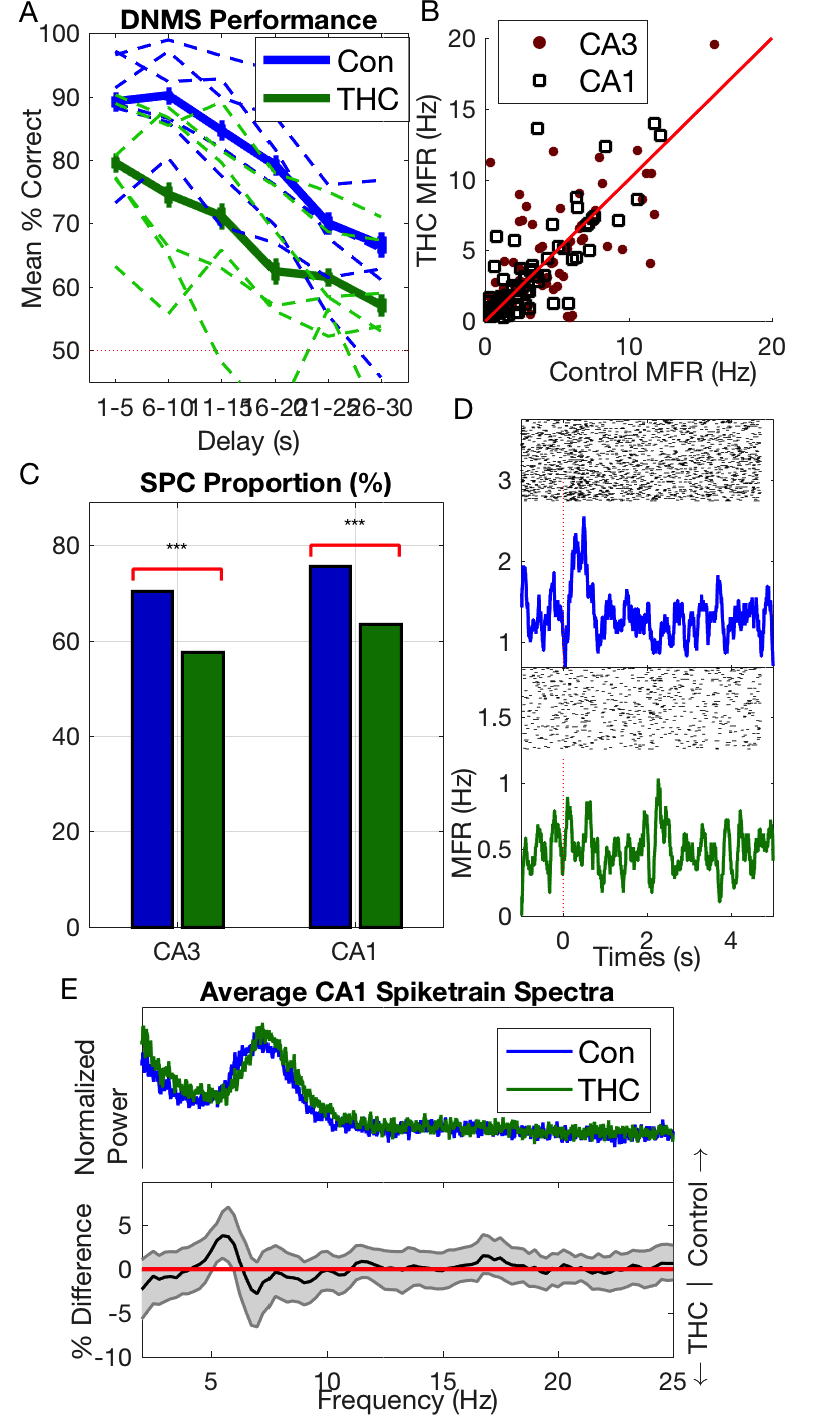
\includegraphics[width=85mm]{sig}
\caption[Signal Analysis]{
(A) Behavioral performance on Delayed-NonMatch-to-Sample (DNMS) task in both control and THC sessions. Dashed lines show individual animal performance, while solid lines show mean performance over all animals. Bars indicate SEM. Dashed red line indicates performance at chance level.
(B) Individual neuron mean firing rate (MFR).
(C) Sample-presentation cell proportion in CA3 and CA1 cells in control \& THC sessions
(D) Example of a sample-presentation cell in a control session (top) which lost its firing specificity under THC (bottom). X-axis shows MFR (Hz)
(E) Average CA1 spiketrain spectra (top). Bottom shows mean difference in \textit{individual} cell spectra (thus it is not simply the difference between the signals in above which are averaged over whole population). Gray error bounds indicate 99\% confidence bounds.
In (B) and (E), only neurons recorded in at least one control \& THC session were included. Results for neurons recorded in several control or THC sessions were averaged over those sessions.}
\label{sig}
\end{figure}


    \subsection{Systems Analysis}

The remainder of the study will focus on systems analysis of the Schaffer collateral synapse  connecting CA3 to CA1, and how this synapse is affected by THC.
Systems analysis aims to identify the input-output "blackbox" by which the input spiketrains are transformed into the output spiketrain.
On a more abstract level, it aims to identify how the information encoded in CA3 is propagated into CA1.
This is distinct from the \textit{signal} analysis done in the previous section which only looks at features of individual spiketrains rather than the causal relationship between multiple spiketrains as done in systems analysis.

The relationship between an arbitrary number of input CA3 spiketrains and the output CA1 spiketrain was modeled using a multivariate autoregressive model described by Eq. \ref{eq:MVAR} and an example of which is pictured in Fig. \ref{ex}a.
Each system consists of $N$ input CA3 neurons and $N$ feedforward filters describing the dynamical input-output relationship between the given CA3 and CA1 neurons (Fig. \ref{ex}b). 
%\footnote{So far used the term "feedforward filter". Maybe "input-output (IO) filter" is better?}.
Intuitively, these filters can be thought of as the EPSP elicited in the output CA1 neuron in response to an action potential (AP) in the input CA3 neuron.
However, unlike EPSPs which traditionally only encapsulate ion-conductances from neurotransmitter-gated ion channels, the "blackbox" nature of the feedforward filters means they also include more complex dynamical effects such as dendritic integration, spike generation, active membrane conductances, and feedforward interneuronal inhibition (thereby allowing the filters between two pyramidal cells to be inhibitory).
Each model also includes a feedback (autoregressive) filter which describes the effects of past output spikes onto the output present.
This filter, which can be intuitively thought of as the afterhyperpotential (AHP) \citep{spruston07} includes intracellular processes such as the absolute and relative refractory periods, slow potassium conductances, and $I_h$ conductances.
It also includes more complex intercellular processes such as the recurrent connections between CA1 pyramidal cells and interneurons \citep{klausberger08}.
Neuronal connectivity was estimated using a stepwise input selection procedure.
Filter parameters were estimated with Laguerre basis regression using neuronal activity around the sample phase.
Model significance was verified using ROC plots and shuffling methods (see supplementary methods).

A representative connectivity grid from a recorded THC session with 10 recorded neurons (4 CA3, 6 CA1) is shown in Fig. \ref{ex}a.
Fig. \ref{ex}b shows a sample system from this session between 3 CA3 pyramidal cells and 1 CA1 pyramidal cell.
Note that two of the feedforward filters are excitatory (above the x-axis) while the third has both excitatory and inhibitory components, presumably arising through feedforward inhibition involving interneurons \citep{pouille01,zemankovics13}.
The system also involves a feedback filter which shows a relatively long refractory period ($\sim$40ms) followed oscillatory bursting activity.
Oscillations in the CA1 pyramidal cell AHP are a well known phenomena caused by slow $K^+$ and $I_h$ conductances, and these oscillations are known to lead to theta resonances \citep{leung98,yarom00,sandler14}.
In order to study the filter oscillations more closely, the filter frequency spectra were plotted in Fig. \ref{ex}c.
Both feedforward excitatory filters were found to have peaks in the high theta range (8-9 Hz).
Intuitively, this can be understood to mean that information encoded in the theta range in these input neurons is preferentially transmitted to the output CA1 neuron.
Furthermore, the feedback filter has a low theta resonance of 3.5 Hz.
Significance metrics for the displayed system is shown in Fig. \ref{SFMCsig}, and additional systems are shown in Fig. \ref{SF_MVARxtra}.
All together 66\% (707/1068) of all systems were found to be significant and 2139 feedforward and 707 feedback filters were obtained.
THC was found to reduce the amount of significant models per session ($\Delta=-7.4\%$, $P=.011$), but the predictive power of significant models, as measured by AUC (see supplementary methods), was unaltered ($P=.24$).

\begin{figure}[!ht]
\centering
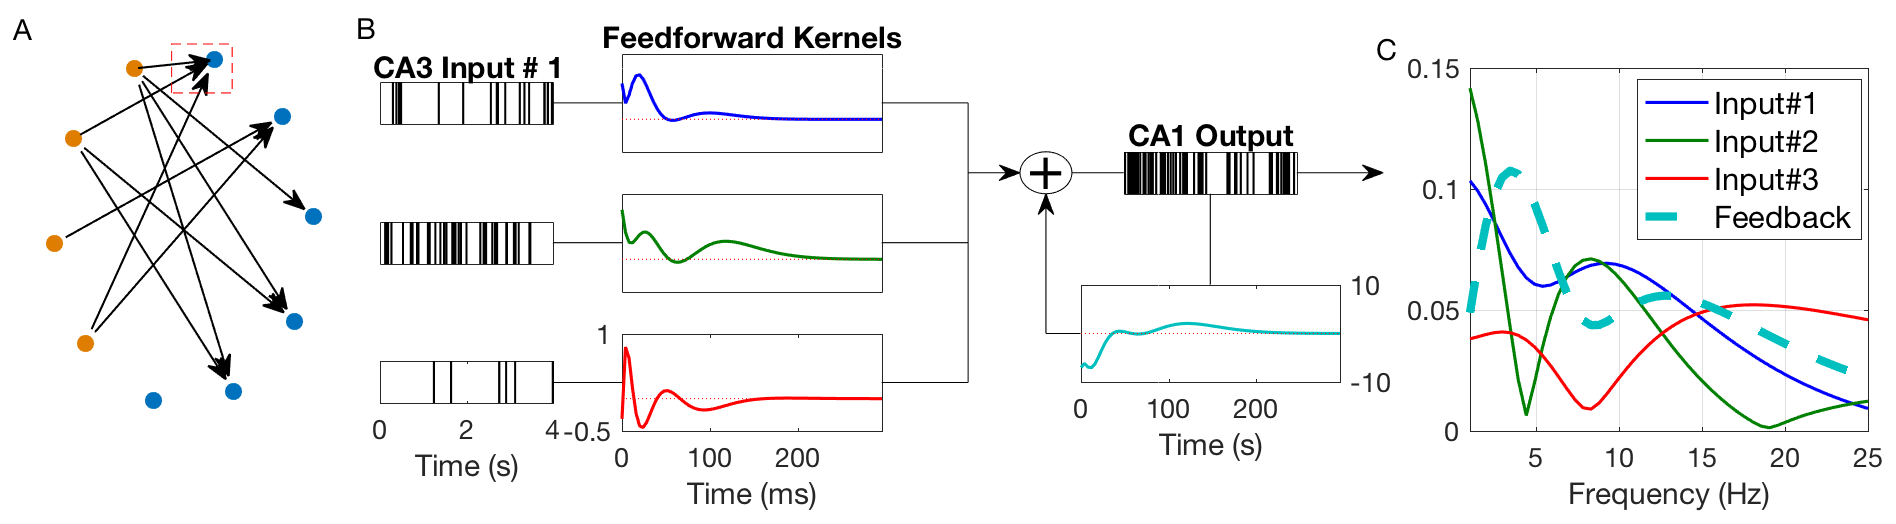
\includegraphics[width=160mm]{ex_tmp}
\caption[Example System]{
(A) Example connectivity grid of 4 CA3 neurons (orange) and 6 CA1 neurons (blue) recorded during a single session. Note that 1 CA1 neuron has no significant granger-causal inputs. Each line represents a causal connection between those neurons, as encapsulated by a feedforward filter.
(B) Example system of CA1 neuron enclosed by the red box in (A). Diagram shows 3 input CA3 spiketrains followed by their respective feedforward filters which are summed with the feedback filter to generate the output CA1 spiketrain. All feedforward filter are plotted with the same y-axis scale. Dashed red line in filter boxes indicates x-axis.
(C) Normalized filter spectra computed of feedforward and feedback filters from (B).}
\label{ex}
\end{figure}

To study how THC affects system dynamics on a population level, we examined how features change in the entire sample of control and THC filters.
The average filter frequency profile for both control and THC sessions is shown in Fig. \ref{ker}a,b (top).
Both feedforward and feedback spectra are found to have clear theta band peaks, thus generalizing the trend seen in the example system of Fig. \ref{ex}.
This is consistent previous reports which show that CA3 propagates strong theta rhythms to CA1 \citep{kocsis99,buzsaki02} and also that CA1 is capable to generating endogenous theta rhythms \citep{williams09}.
THC produced a significant decline in the theta power of the feedback filters ($\Delta=20.8\%$, $P<.001$; Fig. \ref{ker}b).
Note that the feedback filter theta reduction is about 10x stronger than the theta reduction found in the CA1 spiketrain signals (Fig. \ref{sig}e).
No reduction in theta power was found in the feedforward filters ($P=.61$, Fig. \ref{ker}a).
This result suggests that cannabinoid-induced theta desynchronization results primarily from altered feedback properties rather than changes in CA3$\to$CA1 dynamics.

Cannabinoids have been reported to affect network excitation-inhibition balance (EIB) \citep{ozaita12,monory15}.
Particularly, there is much debate whether cannabinoids are pro- or anticonvulsants \citep{hill13,turkanis82,clement03,blair06,rudenko12}.
In order to examine the effects cannabinoids have on network EIB, we quantified the excitation of the estimated filters using a metric called the excitatory index (EI), which is the ratio between positive filter area and total filter area.
It was found that THC had no significant effect on feedforward EI ($P=.14$); however, there was an insignificant trend showing that THC-induced decreases in feedforward EI were correlated with behavioral deficits ($R^2=.27, P=.063$, Fig. \ref{ker}c).
Additionally, THC reduced the amount of casually connected CA3-CA1 neuronal pairs ($\Delta=-8.9\%$, $P<.001$).
These findings, together with the THC-induced decrease of CA3$\to$CA1 significant models, suggest that THC reduces the causal influence CA3 neurons have on CA1 spiketimes.
In other words, THC can be said to functionally isolate CA1 from CA3.
It was also found that THC significantly increased feedback EI ($\Delta=3.5\%$, $P=.022$) and that the increased feedback EI was correlated with behavioral deficits ($R^2=.38, P=.007$, Fig. \ref{ker}d).

\begin{figure}[!ht]
\centering
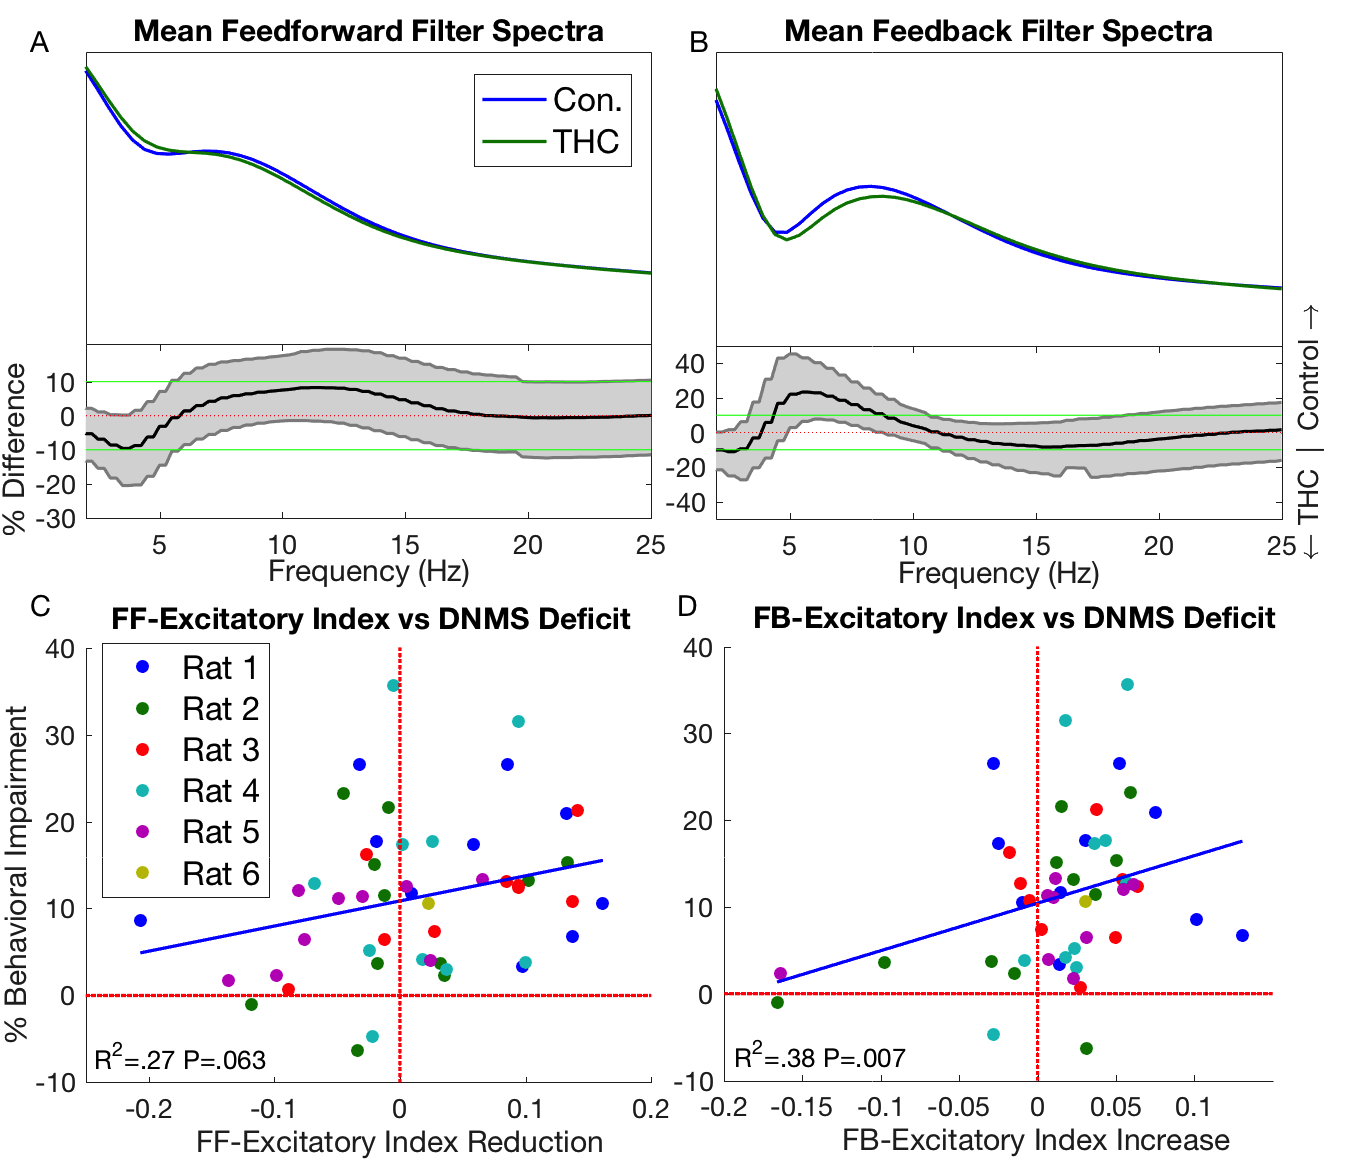
\includegraphics[width=120mm]{ker}
\caption[Kernel Population Metrics]{
Average feedforward (A) and feedback (B) filter spectra in control and THC sessions (top), and their differences (bottom). Same format and analysis as Fig. \ref{sig}a.
(C) Correlation between feedforward filter excitatory index (EI) reduction and behavioral deficits. Each point represents a specific THC session, with points of the same color coming from the same animal. X-axis shows reduction in feedforward EI, while y-axis shows reduction in behavioral performance. Both reductions were taken relative to control sessions (see supplemental methods).
(D) Same as (C) but for feedback EI \textit{increase}.}
\label{ker}
\end{figure}

    \subsection{PDM Analysis}

The large quantity ($>$2800) and variability of the obtained filters describing the CA3$\to$CA1 dynamic transformation presents a challenge of interpretation.
Namely, how could one identify features from the entire filter population which are representative of the CA3$\to$CA1 transformation rather than just the input-output relationship found in this or that particular pair of neurons.
In essence this is an unsupervised learning problem which aims to identify hidden structure within the filter population for the purpose of knowledge discovery.
Our group has developed the concept of the global principal dynamic modes (gPDMs) towards this effort \citep{marm04,marm13,sandler15stc}.
The gPDMs are a system-specific and efficient basis set which contain the essential dynamic components of the filter population and are meant to be amenable to biological interpretation.
One set of gPDMs were estimated from all (control and THC) obtained filters with the hypothesis that THC would primarily change the expression strength of the gPDMs rather than their specific shapes.

Fig. \ref{pdm}a,b shows the obtained feedforward and feedback gPDMs in both the time and frequency domain.
Once again, the feedforward and feedback gPDMs represent the dominant independent componenets of feedforward and feedback kernels, respectively.
The first feedforward gPDM was found to have almost all its energy in the 1st time bin, with an immediate decline thereafter.
This gPDM represents near concurrent firing between CA3 and CA1 neurons and presumably results from both direct CA3$\to$CA1 connections via the Schaffer collateral synapse \citep{deadwyler75,sandler15clpp} and common inputs from the entorhinal cortex \citep{jones93,mehta09}.
The third feedforward gPDM, which is characterized by an initial inhibitory phase, presumably represents feedforward interneuronal inhibition which is prevalent in the CA3$\to$CA1 connection \citep{pouille01,zemankovics13}.
THC was not found to influence the strength of either of these gPDMs ($P=.76$, $P=.60$; Fig. \ref{SFnegpdm}).
The second feedforward gPDM which is characterized by sustained and oscillatory excitation was found to have a strong theta peak in the frequency domain.
Furthermore, it was found that THC-induced declines in the strength of this gPDM were correlated with behavioral deficits ($R^2=.30$, $P=.032$; Fig. \ref{pdm}c).

\begin{figure}[!ht]
\centering
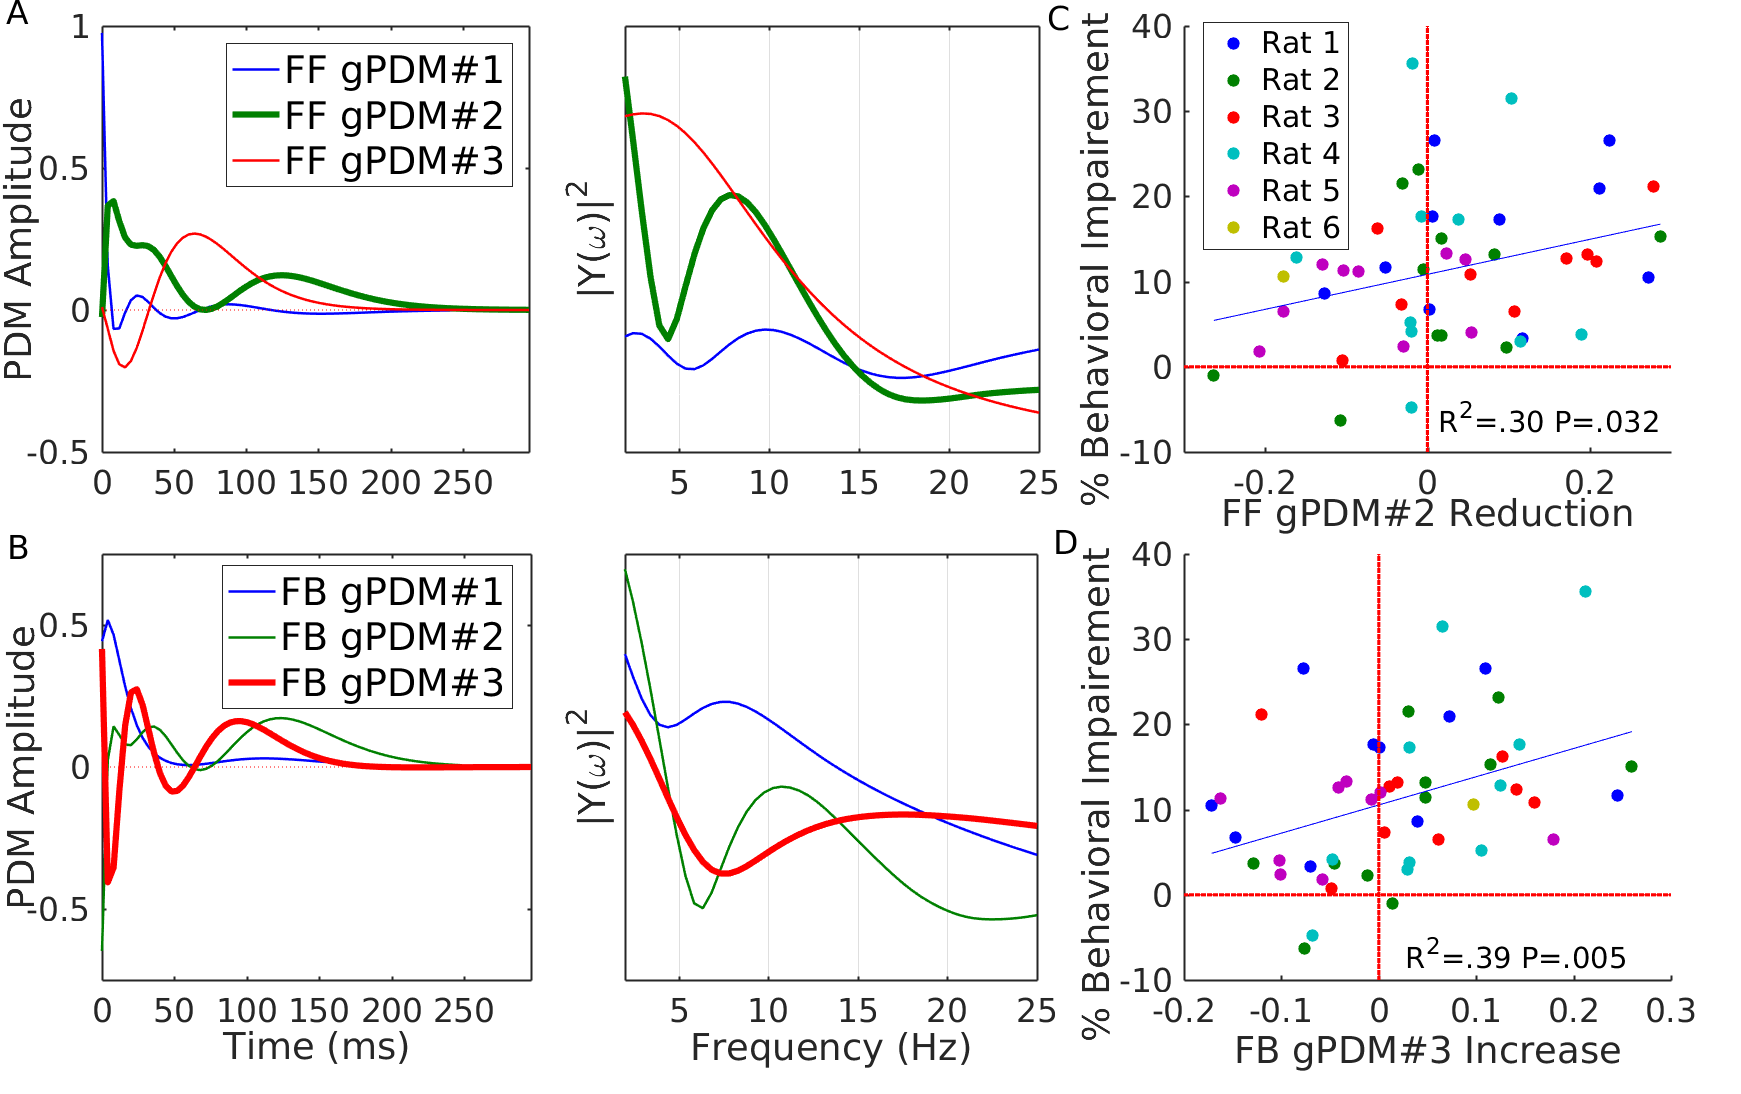
\includegraphics[width=130mm]{pdm}
\caption[PDM Analysis]{
Feedforward (A) and feedback (B) global principal dynamic modes (gPDMs) in both the time (left) and frequency domain (right).
Reductions in 2nd feedforward gPDM (C) and increases in 3rd feedback gPDM (D) were found to be correlated with behavioral deficits. Same format as Fig. \ref{ker}.}
\label{pdm}
\end{figure}

The three obtained feedback gPDMs are shown in Fig. \ref{pdm}b.
These gPDMs express the essential feedback dynamics found in CA1 neurons.
As previously mentioned, these dynamics arise through the combination of intracellular processes such as the AHP and extracellular processes such as recurrent connections between CA1 pyramidal cells and interneurons.
%\footnote{I decided not to force myself to interpret the 1st 2 FB PDMs, since it is not at all obvious what they are. Do you think this is ok?}
It was found that THC-induced increases in the third feedback gPDM were correlated with behavioral deficits ($R^2=.39$, $P=.005$; Fig. \ref{pdm}d).
This correlation was not seen in either of the first two feedback gPDMs ($P=.32$, $P=.75$; Fig. \ref{SFnegpdm}).
Notably, the 3rd feedback gPDM was seen to be "theta-blocking" in the frequency domain due to its trough at 8 Hz. 
This gPDM counteracts the 1st "theta-promoting" feedback gPDM and disrupts theta oscillations in the CA1 neuron.
The THC-induced changes in the feedforward and feedback theta gPDMs paint a more complete picture of the CA1 theta reductions seen in Fig. \ref{sig}e.
Namely, they attribute the theta losses to specific feedforward and feedback dynamical filters which may potentially be traced to specific biophysical mechanisms.
Furthermore, changes in these dynamical filters have been specifically correlated with behavioral deficits, which could not be done with theta reductions in the CA1 signal (Fig. \ref{SFnegsig}).

\section{Discussion \label{disc}}

The current study uses 'data-driven' nonparametric system dynamics modeling tools to study the effects of THC on the Schaffer Collateral synapse in rodents.
The chief findings of the study can be summarized as:
(1) THC induced little or no change in traditional rate and temporal coding metrics such as MFR and theta power, 	
(2) THC altered the CA1 excitatory-inhibitory balance by reducing feedforward influence from CA3 while increasing feedback excitation from CA1,
(3) THC reduced theta information flow through the Schaffer collateral synapse,
and (4) The magnitudes of both of the previous effects were directly correlated with the severity of behavioral deficits induced by THC.
Overall these results suggest the conclusion that THC impairs memory encoding by functionally isolating CA1 from CA3.

From a computational perspective, the nonparamteric modeling methods used in this study proved successful in studying the network level effects of cannabinoids since, unlike biophysical models, all model parameters where estimated directly from recorded data and very few \textit{a priori} assumptions were made about the effects of THC \citep{marm04,song09par1,sandler15}.
The global principal dynamic modes (gPDMs), which were derived from MVAR filters of the entire population of neurons, further extracted hidden dynamical structure from 'noisy' neuron-neuron variability.
Importantly, THC-induced changes in the gPDMs were directly correlated with behavioral impairments, thus justifying their utility.
Furthermore, while most in-vivo studies on THC analyze macro level signals such as ECoG and EEG, this work adds to a relatively small body of literature which analyzes the effects of THC on neuronal population spiking activity.
Finally, to our knowledge, this is the first work which examines the effect of THC on neuronal systems dynamics, or the causal interactions between signals, rather than on neuronal signals themselves.

It was found that THC increased feedback excitatory index in CA1 and that the magnitude of this effect was correlated with behavioral deficits. 
We hypothesize that this is due to reduced feedback inhibition from CA1 cholecystokinin (CCK)-containing basket cells.
While CCK cells only make up only 13.9\% of interneurons \citep{bezaire13}, they express significantly more CB1 receptors than any other cell in the hippocampus \citep{katona00}, and their primary output is to CA1 pyramidal cells \citep{bezaire13}.
Increased THC concentrations would reduce CCK interneuron output by (1) reducing the amount of GABA they release per action potential (2) reducing their MFR due to reduced glutamatergic input from principal cells in both CA3 and CA1 \citep{gulyas04,lee10}.

It was also found that THC reduced the number of casually connected CA3-CA1 neuronal pairs; furthermore there was an interesting but insignificant trend for THC-induced deficits in feedforward excitation to lead to behavioral deficits.
This trend may prove to be significant given a higher sample size. 
We hypothesize that this reduced feedforward influence is caused by decreased glutamate release from CA3 pyramidal cells due to CB1 receptor activation by THC \citep{shen96}.
Even though pyramidal cells have much lower densities of CB1 receptors than interneurons \citep{katona00,ohno02}, there is evidence that CB induced reduction of excitation is larger than these relative densities suggest. 
Principal cells outnumber interneurons 20:1 in CA1 \citep{mehta09} and their CB1 receptors were found to be several fold more efficacious than those of interneurons \citep{steindel13}. 
Further, lower baseline activation levels of CB1 receptors on principal cells than on interneurons suggest they would be disproportionately activated by CB agonists \citep{ruehle12}. 
Altogether, the decreased feedback inhibition and feedforward excitation amount to a functional isolation, or breakdown in information flow between CA3 and CA1.
We suggest that this functional isolation is responsible for the behavioral impairments seen in the DNMS task.

\iffalse
It was found that THC reduces the amount of casually connected CA3-CA1 neuronal pairs; furthermore there was an interesting but insignificant trend for THC-induced deficits in feedforward excitation to lead to behavioral deficits.
%This trend may prove to be significant given a higher sample size. 
We hypothesize that this reduced feedforward influence is caused by decreased glutamate release from CA3 principal cells due to CB1 receptor activation by THC \citep{shen96}.
The reduced feedforward excitation was compensated by increased feedback excitation - an effect which was also correlated with behavioral deficits.
We hypothesize that this is due to decreased drive from CA1 cholecystokinin (CCK)-containing basket cells.
While CCK cells only make up only 13.9\% of interneurons \citep{bezaire13}, they express significantly more CB1 receptors than any other cell in the hippocampus \citep{katona00}, and their primary input and output is from/to CA1 pyramidal cells \citep{bezaire13}.
Increased THC concentrations would reduce CCK output by (1) reducing the amount of GABA they release per action potential and (2) reducing their total amount of action potentials due to reduced glutamatergic input from CA1 pyramidal cells.
Altogether, this would amount to a functional isolation, or breakdown in information flow from CA1 from CA3, thus inducing the behavioral impairments seen in the DNMS task.
Furthermore, the only reason that MFR remained constant is that at the given dosage there was a net balance between these two opposing phenomena.
\fi


The 'functional isolation' hypothesis is further supported by previous work which showed that the behavioral impairments caused by cannabinoids in the DNMS task were similar to those seen with a full pharmacological lesion of the hippocampus \citep{hampson98}
Given the centrality of CA3$\to$CA1 information flow to hippocampal function, a functional isolation of these areas could indeed presumably lead to impairments similar to that of a full lesion.
Relatedly, \citet{goon10} injected THC intraperitoneally at low 1 mg/kg doses as in this study and in higher doses of 3 mg/kg.
They found that while both doses disrupted hippocampal synchrony, only the higher dose resulted in a reduction in pyramidal cell MFR.
This suggests that at the lower dose both previously described phenomena are at a net balance, while at the higher dose, the decrease in feedforward excitation overpowers the increase in feedback excitation and results in lower MFR.
Finally, the hypothesis predicts a breakdown in the normal spiketime coordination between pyramidal cells and interneurons in CA1 circuits.
The breakdown of this coordination, which has been extensively implicated in hippocampal oscillations \citep{traub03,kopell05}, could be responsible for the observed decrease in theta oscillations and information flow.

Although the current results only suggest this hypothesis, several experiments could be done to further substantiate it.
Feedforward and feedback kernels and gPDMs could be estimated at different doses of THC; the hypothesis would predict that different doses would effect the two processes independently, with one of the two processes potentially being more dominant at different THC levels.
Significant developments in in-vivo synaptic patch clamping \citep{tao15} and calcium imaging in recent years could be used to directly measure the drive of CCK cells and CA3 pyramidal cells onto CA1 pyramidal cells under THC.

Much research has been done investigating the effects THC and other cannabinoids have on seizures and epilepsy.
Results so far have been mixed, with various studies showing that THC is both pro- and anticonvulsant \citep{wallace01,blair06,deshpande07,rudenko12,katona15,hill13,katona15}.
The results from this study and the presented hypothesis suggest that THC inherently is not pro- or anti-convulsant but that its effects will depend on the dosage and the unique circuitry of every epileptic focus.
Interestingly, a study by \citet{rudenko12} has shown that indeed the effects of a CB1 agonist were dose dependant, with \textit{lower} doses being anticonvulsant and higher doses being proconvulsant.
Finally, this study suggests that in order to truly understand the effects of THC on epileptic circuits, one must study the systems level changes in circuit dynamics rather than taking a reductionist approach and studying the effects of THC on any particular receptor or cell type.

The present study analyzed the effects of THC from both a signals and systems perspective - and found that systems analysis yielded much richer results.
For example, while analysis of CA1 spiketrain signals showed a slight (2\%) reduction in theta frequency, analysis of system kernels showed that the theta loss was primarily due to CA1 feedback dynamics whose kernels lost over 20\% of their theta power, while theta power in feedforward kernels was unaffected.
Furthermore, only systems analysis allows one to analyze predictive power, feedforward and feedback excitation, and EPSP and AHP waveform shape. Notably, the finding that feedforward influence decreased while feedback excitation increased could not have been observed using only signal analysis which would have only detected a constant MFR.

The present study also employed gPDMs as a means to extract the most significant information from the kernel dynamics estimated from several animals over several sessions \citep{marm04,marm14,sandler14,sandler15clpp}.
The utility of the gPDM method was justified by the finding that reductions in theta related gPDMs in a given session were directly correlated with behavioral deficits, showing that the gPDMs can isolate the particular dynamics which are most affected by THC.
Furthermore, THC-induced theta power losses in spiketrain signals were not found to be correlated with behavioral deficits.
Although in the present study, kernels and gPDMs were restricted to being linear in order to more easily quantify their overall strength and excitation (via the EI), future work will aim to identify the effects of THC on hippocampal nonlinear dynamics \citep{song07,sandler15}.

\section*{Ethics Statement}
All animal protocols were approved by the Wake Forest University Institutional Animal Care and Use Committee, in accordance with the Association for Assessment and Accreditation of Laboratory Animal Care and the National Institute of Health Guide for the Care and Use of Laboratory Animals (NIH Publication No. 8023).

\section*{Acknowledgements}
This work was supported by NIH (www.nih.gov) grant P41-EB001978 to the Biomedical Simulations Resource at the University of Southern California.

\section{Methods \label{meth}}

    \subsection{Experimental Procedures \label{expmeth}}

N=6 Male Long-Evans rats were trained to criterion on a two lever, spatial Delayed NonMatch-to-Sample (DNMS) task (see Fig. \ref{DNMS}).
Briefly, during the sample phase the rat was presented one of two levers (left or right).
After a delay phase ranging from 1-30 seconds, the rat was presented both levers and had to choose the opposite level in order to attain a reward.
Each rodent underwent 16-25 sessions of the task, which were roughly evenly divided between control and THC sessions, wherein the rodent was intraperitoneally administered 1 mg/kg of body weight $\Delta^9$-tetrahydrocannabinol (THC), an exogenous cannabinoid found in marijuana.
During the task, spike trains were recorded in-vivo with multi-electrode arrays implanted in the left and right CA3 and CA1 regions of the hippocampus.
In an effort to acquire a consistent cognitive state, only spiking activity around the sample phase of the task was used.
Spikes from multiple trials were sorted, time-stamped, and concatenated into a discretized binary time series using a 4ms bin.
For more details on the experimental setup, see supplementary methods.

    \subsection{Model Configuration and Estimation}
Nonparametric multiple-input linear autoregressive models were used to model the dynamical transformation between input and output spike trains (see Fig. \ref{ex},\ref{fMVAR}) \citep{sandler14,sandler15}.
Each model consisted of a feedforward component, reflecting the effect of the $N$ input cells on the output cell and a feedback (autoregressive) component reflecting the subthreshold and suprathreshold effects the output cell has on itself. Thus, the output $y(t)$ is calculated as:
\begin{equation}
    y(t)=\sum_{n=1}^{N}\sum_{\tau=0}^{M}k_{n}(\tau)x_{n}(t-\tau)+\sum_{\tau=1}^{M+1}k_{AR}(\tau)y(t-\tau)
\label{eq:MVAR}
\end{equation}
where $k_{n}$ reflects the feedforward filter of input $x_n(t)$, and $k_{AR}$ reflects the feedback filter.
In order to reduce the amount of model parameters and thereby increase parameter stability, we applied the Laguerre expansion technique to expand the feedforward and feedback filters over $L$ Laguerre basis functions (see supplementary methods).

Effective connectivity between neurons was assessed using a Granger causality-like approach.
For each output CA1 neuron, input CA3 neurons were selected in a forward stepwise procedure whereby only neurons which help predict the output CA1 spike activity were included in the model.
After all input neurons were selected, a Monte Carlo approach was used to assess model significance.
A model was deemed significant if the CA3 inputs could predict the output CA1 activity significantly better ($P<.0001$) than randomly permuted versions of the inputs.
See supplementary methods for more details.

\begin{figure}[!ht]
\centering
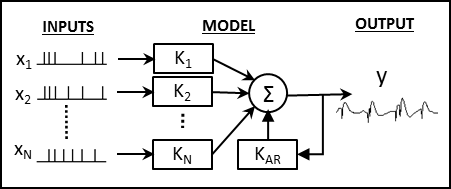
\includegraphics[width=80mm]{MVAR}
\caption[Model configuration schema]{
Model Configuration. Each model has $N$ point-process inputs which each go through a linear filter, $K_i$. These inputs are then summed with the output of the feedback filter, $K_{AR}$ to generate the final output, $y(t)$, which is a continuous signal}
\label{fMVAR}
\end{figure}

    \subsection{Principal Dynamic Modes \label{PDMs}}
The global principal dynamic modes (gPDMs) were obtained in a two step process: first, all filters of each input from every animal were concatenated in a rectangular matrix. Then  singular value decomposition (SVD) was performed on the rectangular matrix to obtain all the significant singular vectors, which are the gPDMs.
It was found that 3 gPDMs were sufficient to describe the linear dynamics both the population of feedforward and feedback filters.
gPDM strength in a given filter was computed by taking the dot product between the gPDM and the filter.
gPDM strength in a given session was computed by taking the average gPDM strength in every filter of that session.



\appendix
\renewcommand\thefigure{S\arabic{figure}} 
\setcounter{figure}{0} 

\section{Supplementary Methods \label{SM}}

All data was previously used in a study on the effects of cannabinoids on hippocampal multifractality \citep{dustin14,dustin15})

    \subsection{Animals}
Subjects were Long–Evans rats (Harlan) aged 4–6 months (n = 6) individually housed and allowed free access to food with water regulation to maintain 85\% of ad libitum body weight during testing.
All animal protocols were approved by the Wake Forest University Institutional Animal Care and Use Committee, in accordance with the Association for Assessment and Accreditation of Laboratory Animal Care and the National Institute of Health Guide for the Care and Use of Laboratory Animals (NIH Publication No. 8023).

    \subsection{Apparatus}
The behavioral testing apparatus for the delayed nonmatch-to-sample (DNMS) task is the same as reported in other studies \citep{hampson00} and consisted of a 43x43x50 cm Plexiglas chamber with two retractable levers (left and right) positioned on either side of a water trough on the front panel.
A nosepoke device (photocell) was mounted in the center of the wall opposite the levers with a cue light positioned immediately above the nosepoke device.
A video camera was mounted on the ceiling and the entire chamber was housed inside a commercially built sound-attenuated cubicle.

    \subsection{DNMS Task}
The DNMS task consisted of three main phases: Sample, Delay and Nonmatch.
The sample phase initiated the trial when either the left or right lever was extended (50\% probability), requiring the animal to press it as the Sample Response (SR).
The lever was then retracted and the Delay phase of the task initiated, as signaled by the illumination of a cue light over the nosepoke photocell device on the wall on the opposite side of the chamber.
At least one nosepoke (NP) was required following the delay interval which varied randomly in duration (1-30 s) on each trial during the session.
The Nonmatch phase began when the delay timed out, the photocell cue light turned off and both the left and right levers on the front panel were extended. Correct responses consisted of pressing the lever in the Nonmatch phase located in the spatial position opposite the SR (nonmatch response: NR). This produced a drop of water (0.4 ml) reward in the trough between the two levers.
After the NR the levers were retracted for a 10.0 second intertrial interval (ITI) before the next Sample lever was presented to begin the next trial.
A lever press at the same position as the SR (match response) constituted an “error” with no water delivery and turned off of the chamber house lights for 5.0s and the next trial was presented 5.0 s later.
Individual performance was assessed as \% NRs (correct responses) with respect to the total number of trials (80-100) per daily (1 hr) sessions.

    \subsection{Drug Preparation \& Administration}
$\Delta^9$-tetrahydrocannabinol (THC) was obtained from the National Institute on Drug Abuse as a 50 mg/ml solution in ethanol.
Detergent vehicle was pre- pared from Pluronic F68 (Sigma, St. Louis, MO), 20 mg/ml in ethanol.
THC was added to the detergent-ethanol solution (0.5 ml of either THC), and then 2.0 ml of saline (0.9\%) was slowly added to the ethanol-drug solution.
The solution was stirred rapidly and placed under a steady stream of nitrogen gas to evaporate the ethanol ($\sim$10 min).
This resulted in a detergent-drug suspension (12.5 mg/ml THC), which was sonicated and then diluted with saline to final injection concentrations (0.5-2.0 mg/ml THC).
On drug administration days, animals were injected intraperitoneally with the drug-detergent solution (1 mg/kg) $\sim$10 min before the start of the behavioral session.
Our experience with these experiments has shown that performance after vehicle injection is not significantly different than no injection, and therefore was omitted during this series of experiments to minimize risk of infection to the animals.
At least two no injection days were imposed between each drug-testing session. All drug solutions were mixed fresh each day.

    \subsection{Surgery}
All surgical procedures conformed to National Institutes of Health and Association for Assessment and Accreditation of Laboratory Animal Care guidelines, and were performed in a rodent surgical facility approved by the Wake Forest University Institutional Animal Care and Use Committee.
After being trained to criterion performance level in the DNMS task animals were anesthetized with ketamine (100 mg/kg) and xylazine (10 mg/kg) and placed in a stereotaxic frame.
Craniotomies (5mm-diameter) were performed bilaterally over the dorsal hippocampus to provide for implantation of 2 identical array electrodes (Neurolinc, New York, NY), each consisting of two rows of 8 stainless steel wires (diameter: 20 $\mu m$) positioned such that the geometric center of each electrode array was centered at co-ordinates 3.4 mm posterior to Bregma and 3.0 mm lateral (right or left) to midline \citep{paxinos86}.
The array was designed such that the distance between two adjacent electrodes within a row was 200 $\mu m$ and between rows was 400 $\mu m$ to conform to the locations of the respective CA3 and CA1 cell layers.
The longitudinal axis of the array of electrodes was angled 30$^{\circ}$ to the midline during implantation to conform to the orientation of the longitudinal axis of the hippocampus, with posterior electrode sites more lateral than anterior sites.
The electrode array was lowered in 25-100 $\mu$m steps to a depth of 3.0 - 4.0 mm from the cortical surface for the longer electrodes positioned in the CA3 cell layer, leaving the shorter CA1 electrodes 1.2 mm higher with tips in the CA1 layer.
Extracellular neuronal spike activity was monitored from all electrodes during surgery to maximize placement in the appropriate hippocampal cell layers.
After placement of the array the cranium was sealed with bone wax and dental cement and the animals treated with buprenorphine (0.01–0.05 mg/kg) for pain relief over the next 4-6 hrs.
The scalp wound was treated periodically with Neosporin antibiotic and systemic injections of penicillin G (300,000 U, intramuscular) were given to prevent infection.
Animals were allowed to recover from surgery for at least 1 week before continuing behavioral testing \citep{berger12}.

    \subsection{Electrophysiological Monitoring \& Preprocessing}
Animals were connected by cable to the recording apparatus via a 32-channel headstage and harness attached to a 40-channel slip-ring commutator (Crist Instruments, Hagerstown, MD) to allow free movement in the behavioral testing chamber.
Single neuron action potentials (spikes) were isolated by time-amplitude window discrimination and computer-identified individual waveform characteristics using a multi-neuron acquisition (MAP) processor (Plexon Inc., Dallas, TX, USA).
Single neuron spikes were recorded daily and identified using waveform and firing characteristics within the task (perievent histograms) for each of the DNMS events (SR, LNP \& NR).
To maintain waveform shape across days, all recorded data was concatenated into one file (separately for each rat) and offline sorting was performed using principal component analysis, peak-valley, and nonlinear energy algorithms in Offline Sorter (Plexon Inc., Dallas, TX, USA).
Hippocampal neuron ensembles used to distinguish recording phases and drug treatment conditions consisted of 10-30 single neurons, each recorded from a separate identified electrode location on either of the bilateral arrays.
All isolated spike trains contained no less than a 1 ms gap at the center of the autocorrelogram.
No effort was made to differentiate between principal cells and interneurons.
Previous work has shown that hippocampal neurons recorded  with the same waveform from the same electrodes exhibit consistent mean, baseline and DNMS task modulated firing rate alterations \citep{deadwyler96,hampson99}, and therefore individual neurons were treated as the same when recorded over multiple days.
A total of 189 neurons recorded during 5,143 recording phases were analyzed in the reported experiments.

    \subsection{Sample-Response Cell Identification}
Prior studies from this laboratory  have  identified  hippocampal neurons recorded as above by “Functional Cell Types” (FCTs) described by different behavioral correlates of DNMS task-related events such as lever position and/or phase of the task \citep{hampson99,goon10}.
Sample-response cells, a subtype of FCTs, were identified by first constructing a smoothed (51 bin) perievent histogram around the sample presentation phase of the DNMS task.
The neurons background firing rate mean and variance were calculated from activity 3.5-5s after sample presentation.
If the neuron's MFR from the 2 second window around sample presentation was 4 standard deviations greater than its MFR from the background period it was classified as a sample-response cell.
It should be noted that for the purpose of this paper other FCTs such as those which respond to a specific lever (left/right) or trial-type cells were not considered \citep{hampson12b}.

    \subsection{Laguerre Expansion Technique}  %go into more details on volterra model here

In order to apply the Laguerre expansion technique \citep{marm04}, the input and output data records were first convolved with the Laguerre functions:
\begin{equation}
    v_{x_{i}}^{(l)}=\sum_{\tau=0}^{M}b_{l}(\tau)x_{i}(t-\tau)
\end{equation}
\begin{equation}
    v_{y}^{(l)}=\sum_{\tau=0}^{M}b_{l}(\tau)y(t-\tau)
\end{equation}
where $b_{l}$ is the $l^{th}$ Laguerre basis function.
By first convolving with the Laguerre basis functions, the dynamical effects of the past input epochs are removed and we are left with a simple regression of contemporaneous data.
Substituting the above equations into equation \ref{eq:MVAR}, we have:
\begin{equation}
    y(t)=k_{0}+\sum_{n=1}^{N}\sum_{l=1}^{L}c_{l,x_{i}}(l)v_{l,x_{i}}(t)+\sum_{l=1}^{L}c_{l,y}(l)v_{l,y}(t)
\label{eq:LET}
\end{equation}
where $c_{l,x_{i}}$ and $c_{l,y}$ are the feedforward and feedback Laguerre expansion coefficients.
To estimate model parameters, eq. \ref{eq:LET} was cast in matrix form:
\begin{equation}
    \bm{y}=\bm{Vc}+\epsilon
\label{eq:mat}
\end{equation}
where $\bm{y}$ is the vector of all $N$ output samples, $\bm{V}$ is the design matrix consisting of the convolved inputs, $\bm{c}$ are the model parameters to be estimated, and $\epsilon$ is the modeling error.
Eq. \ref{eq:mat} was solved using least squares regression (LSR).
%It was found that using the more sophisticated GLM methodology \citep{truccolo05} did not provide significantly more predictive power as measured by $R^2$ and AUC, and significantly increased computational burden, and thus was not adopted.
The memory of our system was fixed at 300ms, in accordance with previous studies \citep{song07,lu11}.
The Laguerre parameter $\alpha$ was fixed at 0.6 to reflect this system memory \citep{marm04}.

    \subsection{Model Selection}
In theory, the most predictive model would include all recorded inputs.
However, such a model would be susceptible to overfitting, and would not reveal which neurons are causally connected to each other.
To overcome this issue a forward step-wise selection procedure was used to minimize overfitting and prune out all inputs which are not causally related to the output \citep{song09}.
Given an output cell and $M$ potential input cells recorded during the same session, the following steps were used to select the $N$ input cells which are causally connected to the output cell.
First, the data was divided into training (in-sample) and testing (out-of-sample) sets.
Then, $M$ single-input single-output (SISO) models were constructed with each of the potential inputs.
The model whose predicted output had the highest correlation, as measured by the Pearson correlation-coefficient, $\rho$, with the actual output was selected. Afterwards, N-1 models were constructed with two inputs: the previously selected input and one of the remaining potential inputs.
If any of the inputs were able to raise $\rho$, the input which raised $\rho$ the most was selected; otherwise, the procedure was ended, and only 1 input was selected.
This procedure was repeated until either none of the inputs were able to raise $\rho$, or all $M$ potential neurons were selected. The $N$ selected neurons were then used as the model input.

    \subsection{Model Validation}
To avoid overfitting, Monte Carlo style simulations were used to select those models which represent significant causal connections between input and output neurons and do not just fit noise \citep{zanos08}.
The following procedure was used: in each run the real input was randomly permuted with respect to the output.
A model was then generated between the permuted input and the real output, and the Pearson correlation coefficient, $\rho_{i}$, was obtained as a metric of performance.
T=40 such simulations were conducted for each output and a set of performance metrics, $\{\rho_{i}\}_{i}^{T}$, was obtained.
Then, using Fisher's transformation, we tested the hypothesis, $H_{0}$, that $\rho$ was within the population of $\{\rho_{i}\}$.
If this hypothesis could be rejected at the 99.99\% significance level, the model was deemed significant.
The very conservative threshold ($P<.0001$) was used due to the large amount of comparisons being made.

    \subsection{Statistical Analysis}
Unless otherwise noted, the unpaired Mann-Whitney U test was used to access whether significant differences exist between two samples. This test was used since it does not assume a normal distribution, and much of our data was found to be skewed/nonnormal. Shift estimates (Hodges-Lehman) and confidence intervals were estimated as prescribed by \citet{higgins93}. In order to estimate the scale estimate, or the ratio between two samples, the data was first log-transformed and then scale estimate was taken to be the antilog of the shift estimate. The $\chi^2$ test was used to compare proportions.

In addition to the Pearson correlation coefficient, $\rho$, Receiver Operating Characteristic (ROC) curves were used to visualize model performance. ROC curves plot the true positive rate against the false positive rate over the putative range of threshold values for the continuous output, y \citep{zanos08}. The area under the curve (AUC) of ROC plots are used as a performance metric of the model, and have been shown to be equivalent to the Mann-Whitney two sample statistic \citep{hanely1982}. The AUC ranges from 0 to 1, with 0.5 indicating a random predictor and higher values indicating better model performance. The $\rho$ and AUC metrics were chosen as they measure the similarity between a continuous 'prethreshold' signal and a spike train. The continuous 'prethreshold' signal was chosen over adding a threshold trigger and comparing true output spike train with an output 'postthreshold' spike train for two reasons. First, this allows us to avoid specifying the threshold trigger value, which relies on the somewhat arbitrary tradeoff between true-positive and false-negative spikes \citep{marm13}. Also, similarity metrics between two spike trains often require the specification of a 'binning parameter' to determine the temporal resolution of the metric \citep{vanrossum01,victor97}.
%\footnote{I should probably add sections on how behavioral correlation analysis \& FFT was done...}


\section{Supplementary Figures \label{SF}}

\begin{figure}[!ht]
\centering
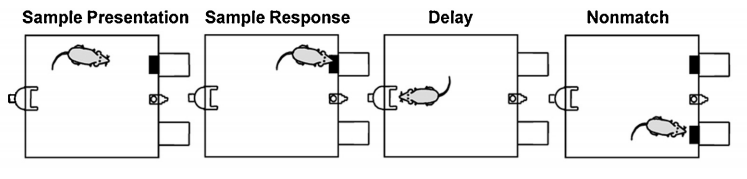
\includegraphics[width=90mm]{DNMS}
\caption[DNMS Task Schematic]{
Schematic of the DNMS task. First the rat is presented with one of two levers (sample presentation), which it presses (sample response). Then following a delay phase, the rat is presented with both levers (Nonmatch), of which it must press the opposite level from which it was presented in order to successfully complete the task. }
\label{DNMS}
\end{figure}

\begin{figure}[!ht]
\centering
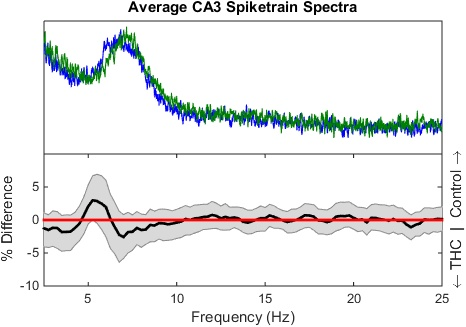
\includegraphics[width=90mm]{SFca3spectra}
\caption[CA3 Frequency Spectra]{
CA3 spectra mean frequency and differences. Same format as Fig. \ref{sig}e. A weak but significant trend was found for declining CA3 theta oscillations ($\Delta=1.94\%$, $P=.045$).}
\label{SFca3spectra}
\end{figure}

\begin{figure}[!ht]
\centering
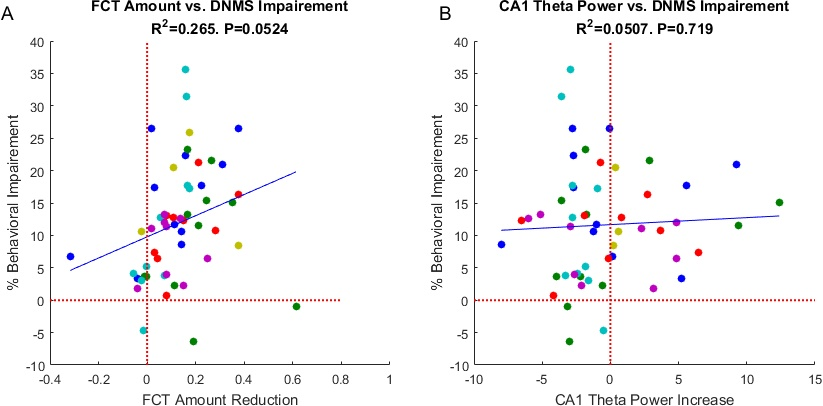
\includegraphics[width=120mm]{SFnegsig}
\caption[Negative CA1 Theta Power Results]{
(A) An insignificant trend was found between the THC-induced decrease in the mean number of sample-presentation cells and behavioral performance ($R^2=.265$, $P=.052$).
(B) No relationship was found between reductions in CA1 theta power and behavioral impairment ($P=.67$).
Format is same as Fig. \ref{ker}.}
\label{SFnegsig}
\end{figure}

\begin{figure}[!ht]
\centering
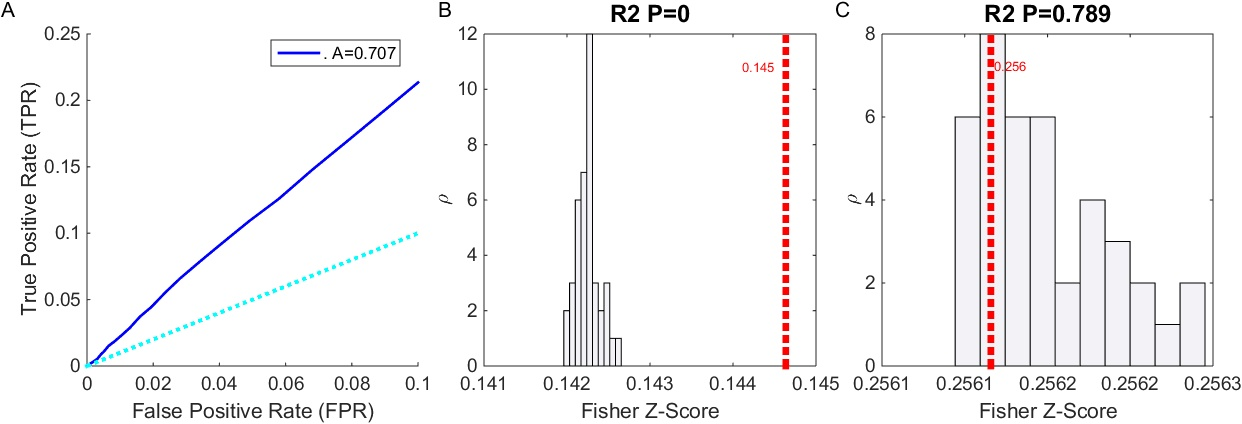
\includegraphics[width=150mm]{SFMCsig}
\caption[MonteCarlo Significance Results]{
(A) ROC plot (see supplementary methods) for model shown in Fig. \ref{ex} showing model predictive power. The light blue line (TPR=FPR) indicates a model with no predictive power.
(B,C) Examples of Monte Carlo simulations: For each model, 40 surrogate models with shuffled inputs were generated. The Fisher z-scores of these models, which are derived from $\rho$,  were plotted as a histogram, while the true $\rho$ value is the plotted dashed red line. The P value for the hypothesis that the true $\rho$ value is greater than the simulated $\rho$ values is printed above the graphs. Models were deemed significant if $P<.0001$. (B) shows the results for the model in Fig. \ref{ex}, which was deemed significant. (C) shows an insignificant model}
\label{SFMCsig}
\end{figure}

\begin{figure}[!ht]
\centering
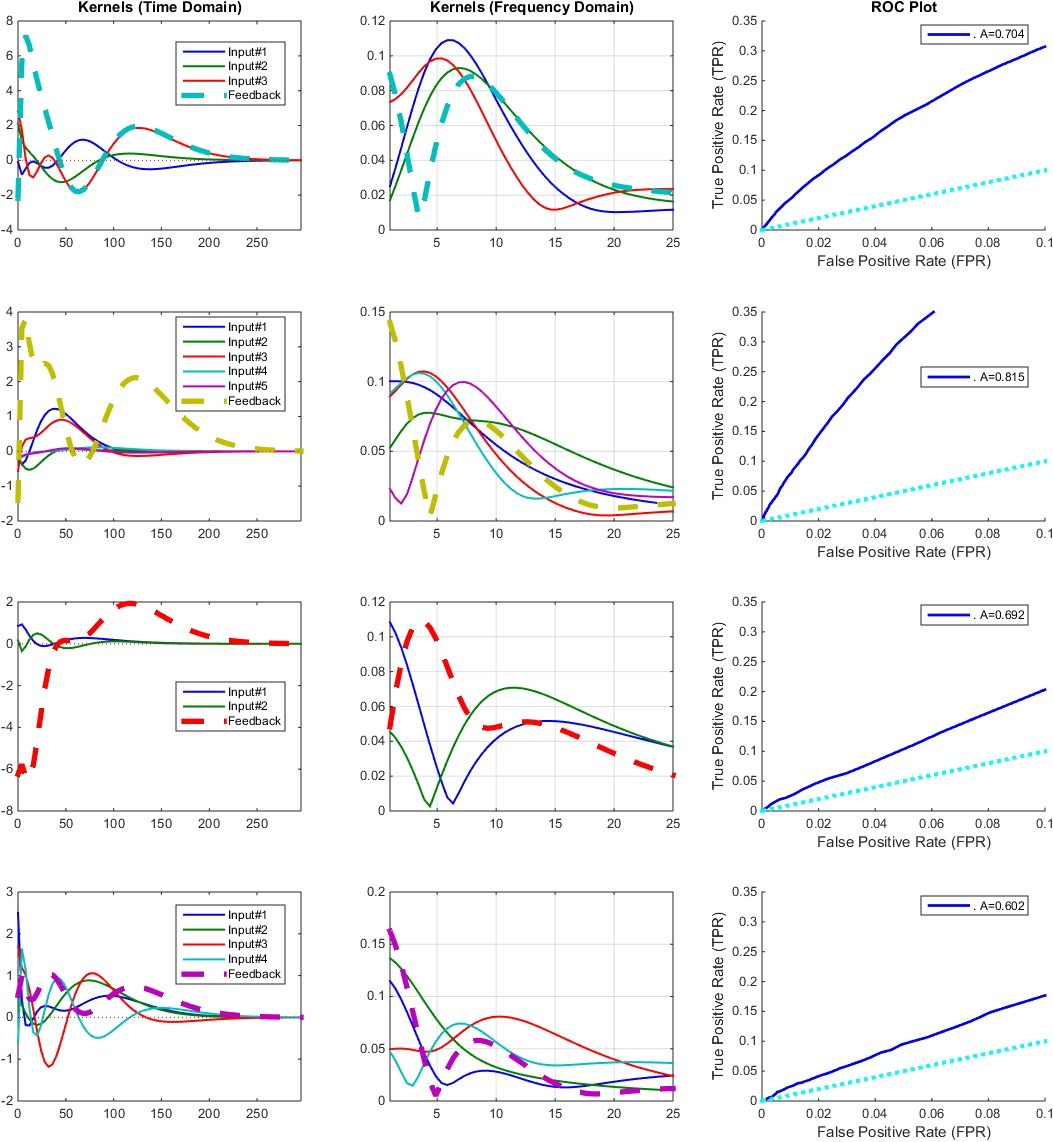
\includegraphics[width=150mm]{SF_MVARxtra}
\caption[Additional System Examples]{
4 additional systems are presented.
Left column shows all system filters, including feedback filter (dashed line) in the time domain.
Middle column shows the filters in the frequency domain and right column shows the ROC plots of the models.
All these models were found to have significant predictive power in Monte Carlo tests.}
\label{SF_MVARxtra}
\end{figure}

\begin{figure}[!ht]
\centering
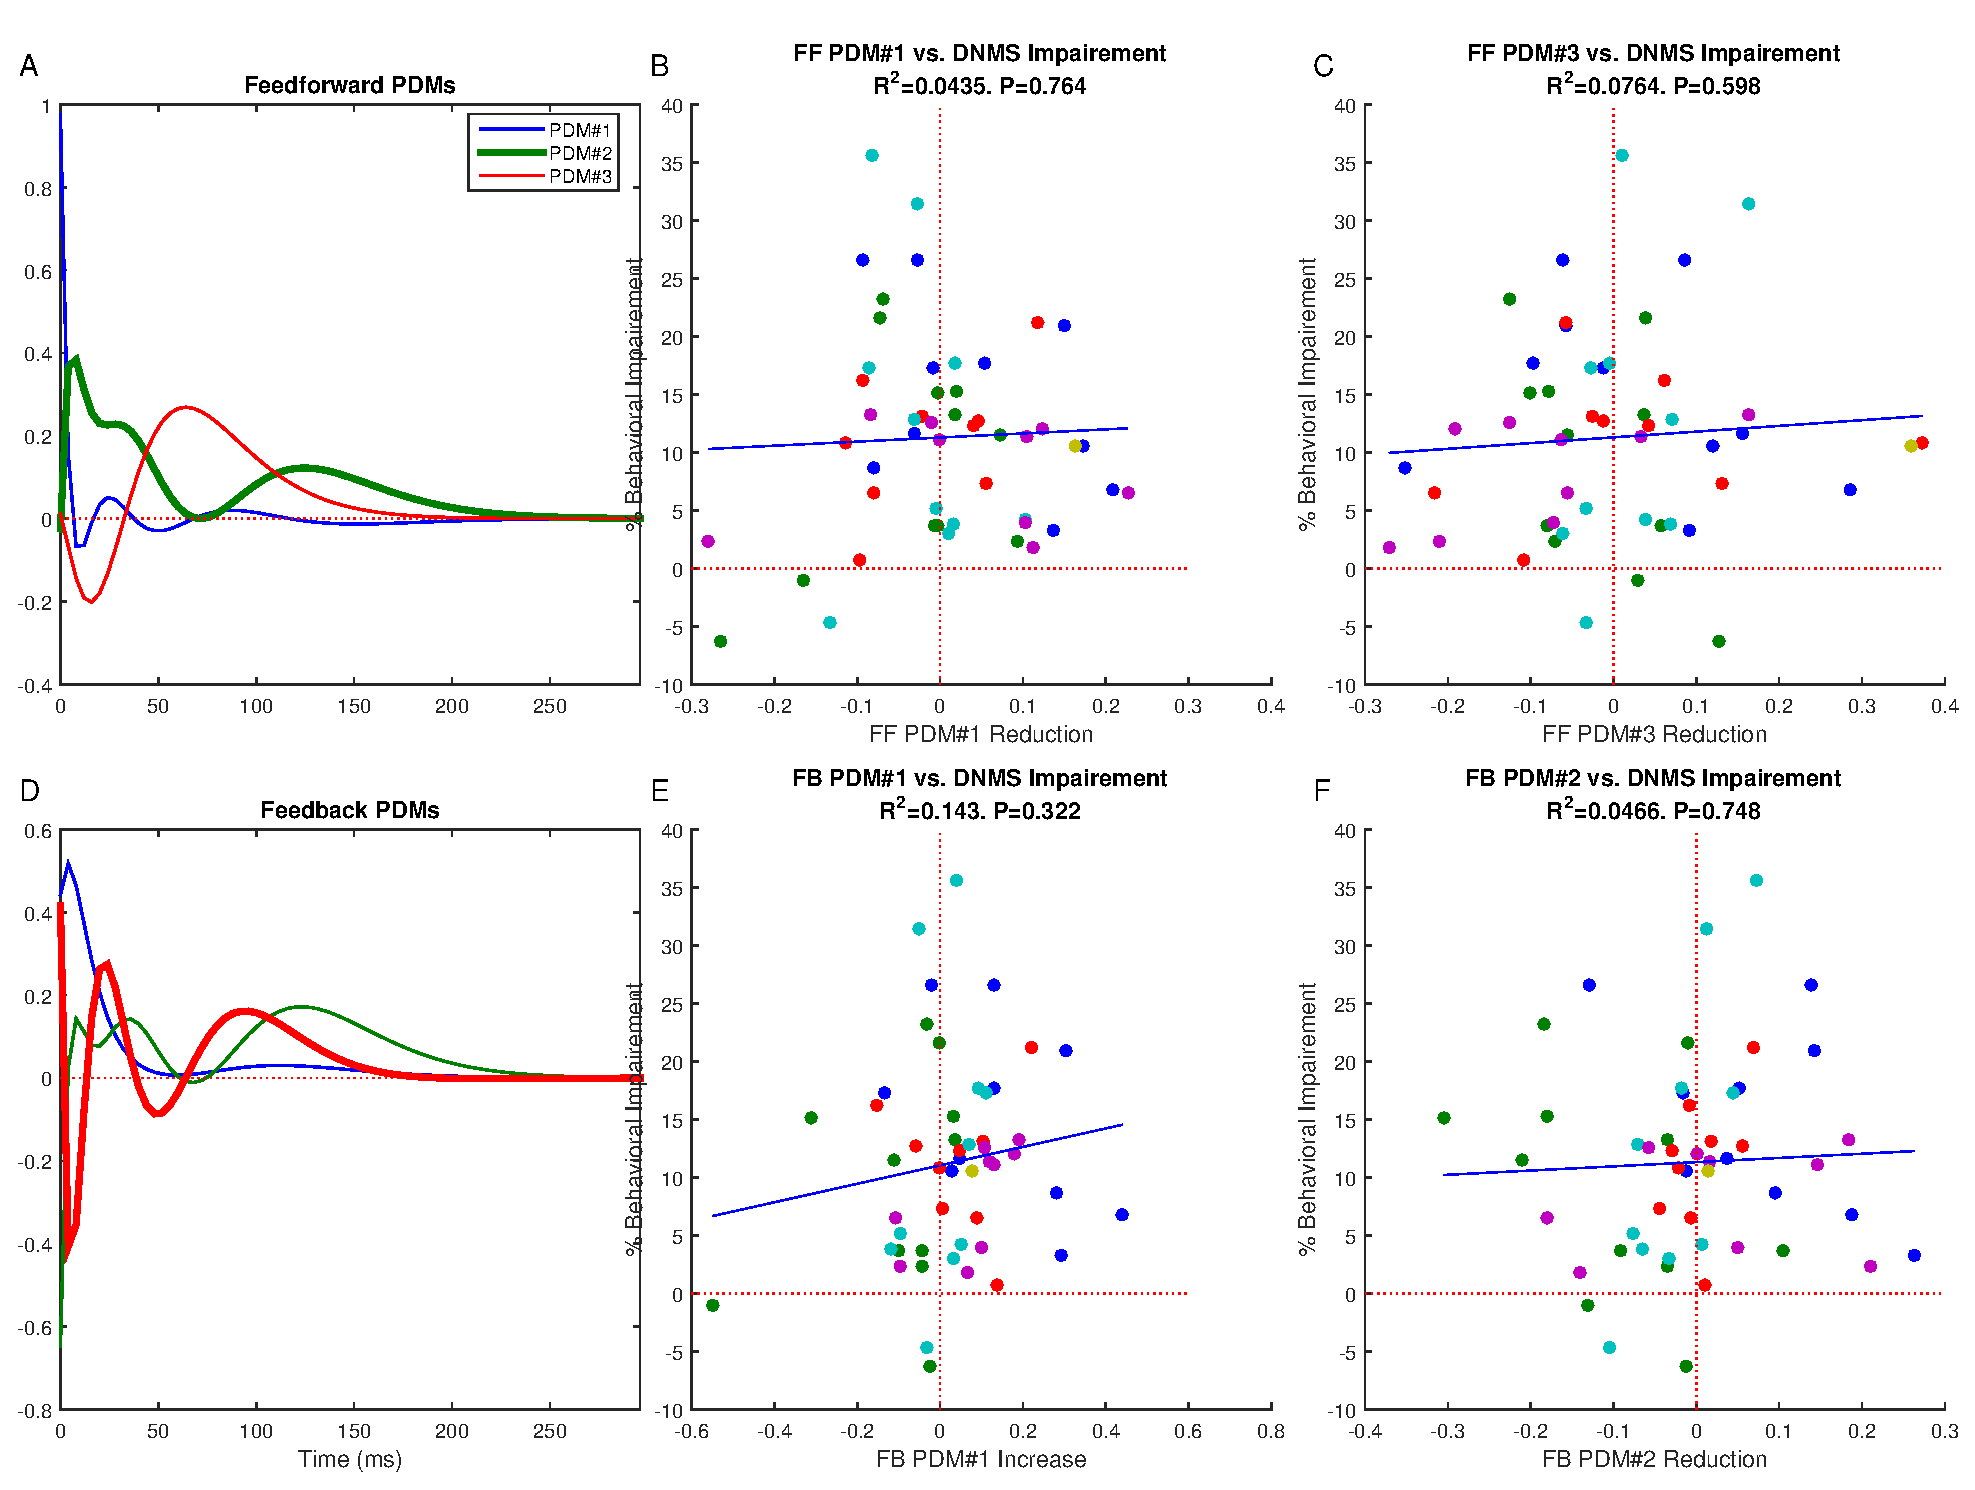
\includegraphics[width=150mm]{SFnegpdm}
\caption[Negative PDM Results]{
Top Row: neither the first (middle column) nor third feedforward gPDM were found to be significantly correlated with THC induced behavioral deficits.
Bottom Row: neither the first (middle column) nor second feedback gPDM were found to be significantly correlated with THC induced behavioral deficits.
Format is same as Fig. \ref{ker}.}
\label{SFnegpdm}
\end{figure}


\clearpage
%\bibliographystyle{plainnat}   %alphabetical
\bibliographystyle{unsrtnat}    %by order of appearance
\bibliography{THCbib,biblio}
                        %C:\Users\Administrator\Documents\Thesis\THESIS_Latex

\end{document} 